\documentclass[11pt]{article}
\usepackage[margin=1in]{geometry}
\usepackage{tikz}
\usepackage{pgfplots}
\usepackage{xcolor}
\pgfplotsset{compat=1.17}

% Color definitions
\definecolor{ropecolor}{RGB}{46, 204, 113}    % Green for RoPE
\definecolor{dropecolor}{RGB}{231, 76, 60}    % Red for DroPE
\definecolor{querycolor}{RGB}{52, 152, 219}   % Blue
\definecolor{keycolor}{RGB}{155, 89, 182}     % Purple
\definecolor{valuecolor}{RGB}{241, 196, 15}   % Yellow

\title{DroPE Activation Analysis: TikZ Figures}
\author{Generated from FINDINGS.md}
\date{}

\begin{document}
\maketitle

%% ============================================
%% FIGURE 1: Massive Value Counts
%% ============================================
\begin{figure}[htbp]
\centering
\begin{tikzpicture}
\begin{axis}[
    ybar,
    width=0.9\columnwidth,
    height=6cm,
    bar width=12pt,
    ylabel={Massive Value Count},
    symbolic x coords={Query,Key,Value},
    xtick=data,
    x tick label style={font=\small},
    legend style={at={(0.5,1.02)},anchor=south,legend columns=2,font=\small},
    ymin=0,ymax=1800,
    ymajorgrids=true,
    grid style=dashed,
    every axis plot/.append style={fill opacity=0.8},
    error bars/.cd,
    y dir=both,
    y explicit,
]
\addplot[fill=ropecolor] coordinates {
    (Query,1476) +- (0,23)
    (Key,1497) +- (0,70)
    (Value,174) +- (0,11)
};
\addplot[fill=dropecolor] coordinates {
    (Query,901) +- (0,36)
    (Key,1332) +- (0,74)
    (Value,177) +- (0,6)
};
\legend{RoPE,DroPE}
\end{axis}
\end{tikzpicture}
\caption{Massive value counts across Q, K, V tensors. DroPE shows 39\% reduction in Query, 11\% in Key. Error bars show $\pm$1 std across 10 samples.}
\label{fig:massive_counts}
\end{figure}

%% ============================================
%% FIGURE 2: Layer 1 Anomaly
%% ============================================
\begin{figure}[htbp]
\centering
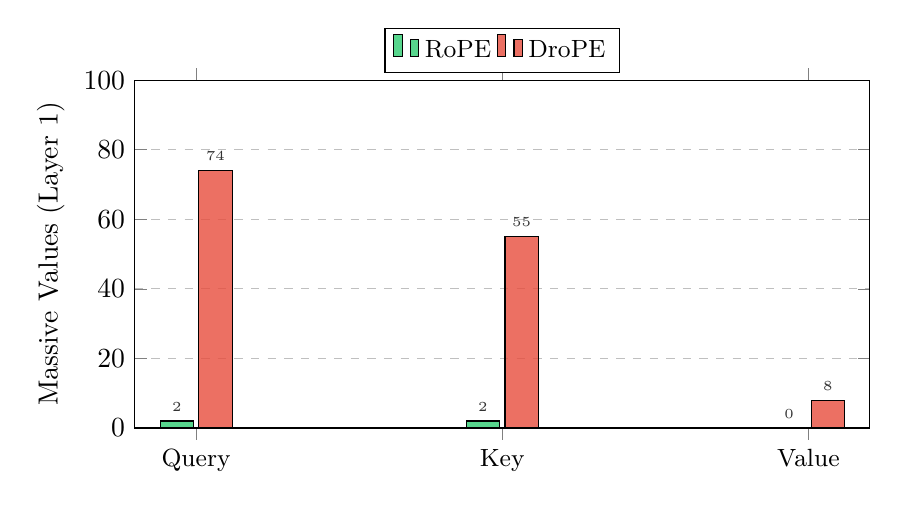
\begin{tikzpicture}
\begin{axis}[
    ybar,
    width=0.9\columnwidth,
    height=6cm,
    bar width=12pt,
    ylabel={Massive Values (Layer 1)},
    symbolic x coords={Query,Key,Value},
    xtick=data,
    x tick label style={font=\small},
    legend style={at={(0.5,1.02)},anchor=south,legend columns=2,font=\small},
    ymin=0,ymax=100,
    ymajorgrids=true,
    grid style=dashed,
    every axis plot/.append style={fill opacity=0.8},
    nodes near coords,
    nodes near coords style={font=\tiny},
]
\addplot[fill=ropecolor] coordinates {(Query,2) (Key,2) (Value,0)};
\addplot[fill=dropecolor] coordinates {(Query,74) (Key,55) (Value,8)};
\legend{RoPE,DroPE}
\end{axis}
\end{tikzpicture}
\caption{Layer 1 Anomaly: DroPE has 37$\times$ more Query massive values at Layer 1 (74 vs 2). The concentration has \textit{moved}, not disappeared.}
\label{fig:layer1_anomaly}
\end{figure}

%% ============================================
%% FIGURE 3: Perplexity After Disruption
%% ============================================
\begin{figure}[htbp]
\centering
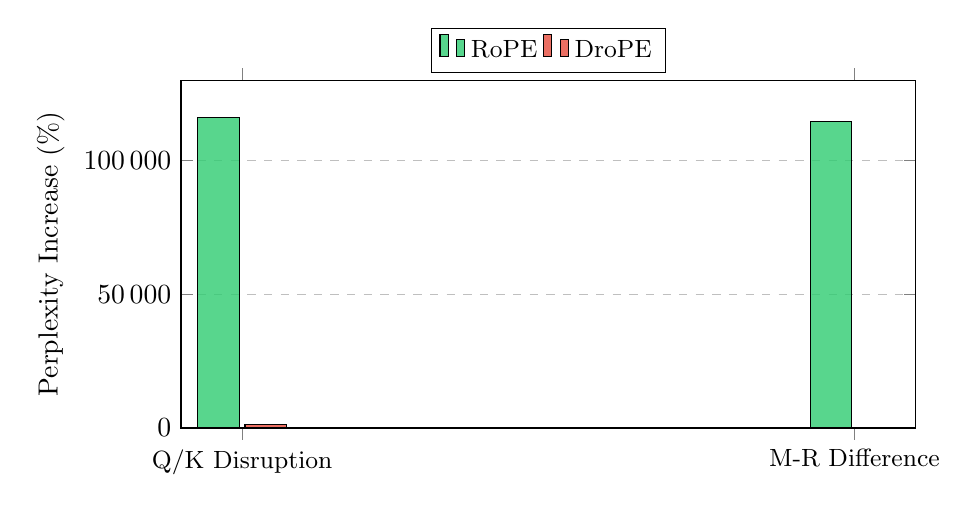
\begin{tikzpicture}
\begin{axis}[
    ybar,
    width=0.9\columnwidth,
    height=6cm,
    bar width=15pt,
    ylabel={Perplexity Increase (\%)},
    symbolic x coords={Q/K Disruption,M-R Difference},
    xtick=data,
    x tick label style={font=\small},
    legend style={at={(0.5,1.02)},anchor=south,legend columns=2,font=\small},
    ymin=0,ymax=130000,
    ymajorgrids=true,
    grid style=dashed,
    every axis plot/.append style={fill opacity=0.8},
    scaled y ticks=false,
    yticklabel style={/pgf/number format/fixed,/pgf/number format/1000 sep={\,}},
]
\addplot[fill=ropecolor] coordinates {(Q/K Disruption,115929) (M-R Difference,114508)};
\addplot[fill=dropecolor] coordinates {(Q/K Disruption,1421) (M-R Difference,0)};
\legend{RoPE,DroPE}
\end{axis}
\end{tikzpicture}
\caption{Perplexity after disrupting massive values. RoPE: +115,929\%. DroPE: +1,421\%. RoPE depends on massive values 82$\times$ more than DroPE.}
\label{fig:ppl_disruption}
\end{figure}

%% ============================================
%% FIGURE 4: Functional Task Degradation
%% ============================================
\begin{figure}[htbp]
\centering
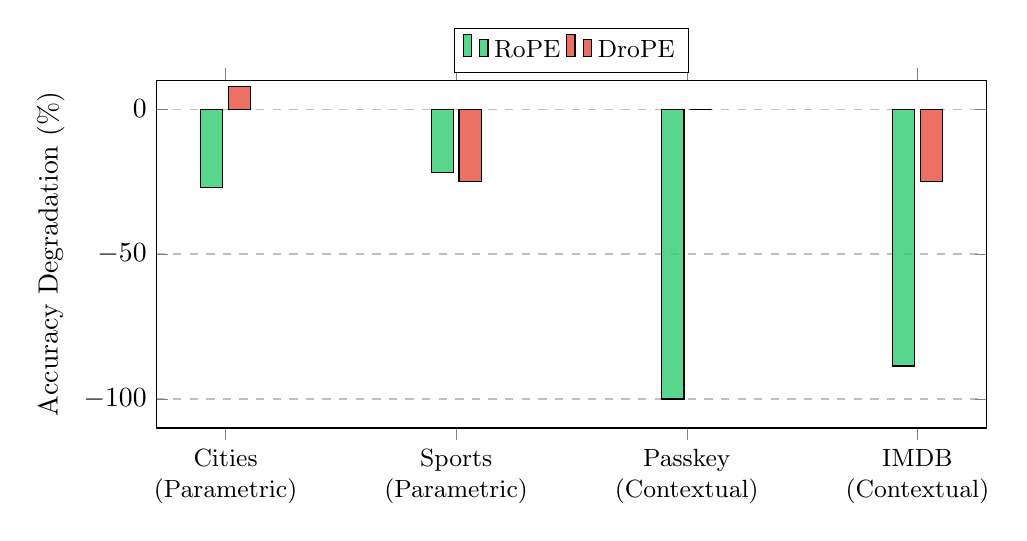
\begin{tikzpicture}
\begin{axis}[
    ybar,
    width=\columnwidth,
    height=6cm,
    bar width=8pt,
    ylabel={Accuracy Degradation (\%)},
    symbolic x coords={Cities,Sports,Passkey,IMDB},
    xtick=data,
    xticklabels={Cities\\(Parametric),Sports\\(Parametric),Passkey\\(Contextual),IMDB\\(Contextual)},
    x tick label style={font=\small,align=center},
    legend style={at={(0.5,1.02)},anchor=south,legend columns=2,font=\small},
    ymin=-110,ymax=10,
    ymajorgrids=true,
    grid style=dashed,
    every axis plot/.append style={fill opacity=0.8},
]
\addplot[fill=ropecolor] coordinates {(Cities,-27.1) (Sports,-21.9) (Passkey,-100) (IMDB,-88.6)};
\addplot[fill=dropecolor] coordinates {(Cities,7.7) (Sports,-25) (Passkey,0) (IMDB,-25)};
\legend{RoPE,DroPE}
\end{axis}
\end{tikzpicture}
\caption{Task accuracy degradation after Q/K disruption. RoPE collapses on contextual tasks (88--100\%). DroPE is robust, especially on Passkey (0\% degradation). Cities accuracy actually \textit{improves} for DroPE.}
\label{fig:task_degradation}
\end{figure}

%% ============================================
%% FIGURE 5: Passkey Retrieval Comparison
%% ============================================
\begin{figure}[htbp]
\centering
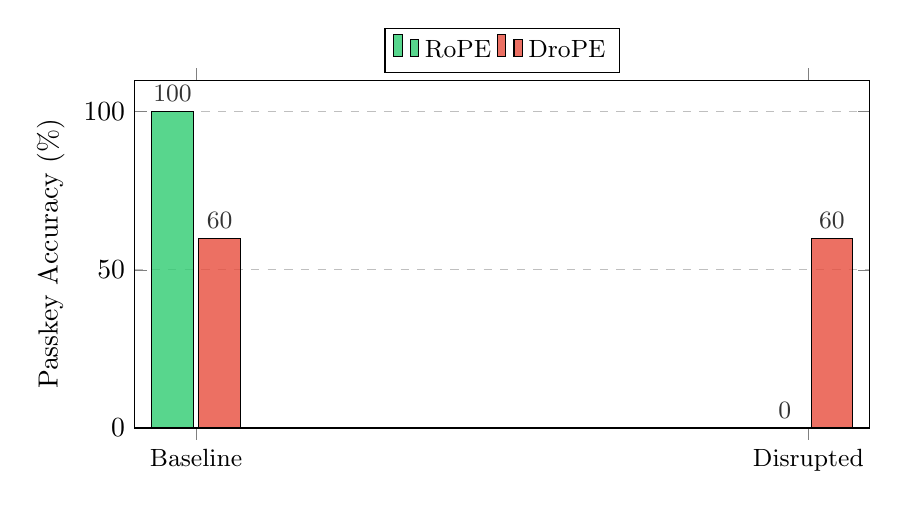
\begin{tikzpicture}
\begin{axis}[
    ybar,
    width=0.9\columnwidth,
    height=6cm,
    bar width=15pt,
    ylabel={Passkey Accuracy (\%)},
    symbolic x coords={Baseline,Disrupted},
    xtick=data,
    x tick label style={font=\small},
    legend style={at={(0.5,1.02)},anchor=south,legend columns=2,font=\small},
    ymin=0,ymax=110,
    ymajorgrids=true,
    grid style=dashed,
    every axis plot/.append style={fill opacity=0.8},
    nodes near coords,
    nodes near coords style={font=\small},
]
\addplot[fill=ropecolor] coordinates {(Baseline,100) (Disrupted,0)};
\addplot[fill=dropecolor] coordinates {(Baseline,60) (Disrupted,60)};
\legend{RoPE,DroPE}
\end{axis}
\end{tikzpicture}
\caption{Passkey retrieval: pure contextual task. RoPE collapses from 100\% to 0\% under disruption. DroPE is completely unaffected (60\% $\rightarrow$ 60\%).}
\label{fig:passkey}
\end{figure}

%% ============================================
%% FIGURE 6: BOS-MLP Ablation
%% ============================================
\begin{figure}[htbp]
\centering
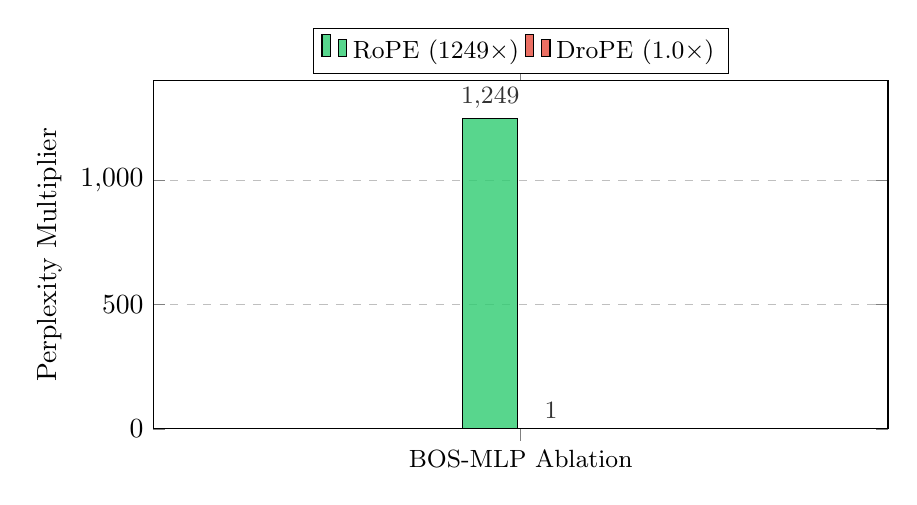
\begin{tikzpicture}
\begin{axis}[
    ybar,
    width=0.9\columnwidth,
    height=6cm,
    bar width=20pt,
    ylabel={Perplexity Multiplier},
    symbolic x coords={BOS-MLP Ablation},
    xtick=data,
    x tick label style={font=\small},
    legend style={at={(0.5,1.02)},anchor=south,legend columns=2,font=\small},
    ymin=0,ymax=1400,
    ymajorgrids=true,
    grid style=dashed,
    every axis plot/.append style={fill opacity=0.8},
    nodes near coords,
    nodes near coords style={font=\small},
]
\addplot[fill=ropecolor] coordinates {(BOS-MLP Ablation,1249)};
\addplot[fill=dropecolor] coordinates {(BOS-MLP Ablation,1.0)};
\legend{RoPE (1249$\times$),DroPE (1.0$\times$)}
\end{axis}
\end{tikzpicture}
\caption{BOS-MLP ablation effect. RoPE perplexity explodes 1249$\times$. DroPE is completely unaffected (1.0$\times$). Both models have similar attention sink rates ($\sim$97\%), but only RoPE depends on BOS-MLP processing.}
\label{fig:bos_mlp}
\end{figure}

%% ============================================
%% FIGURE 7: Layer 1 Architecture Inversion
%% ============================================
\begin{figure}[htbp]
\centering
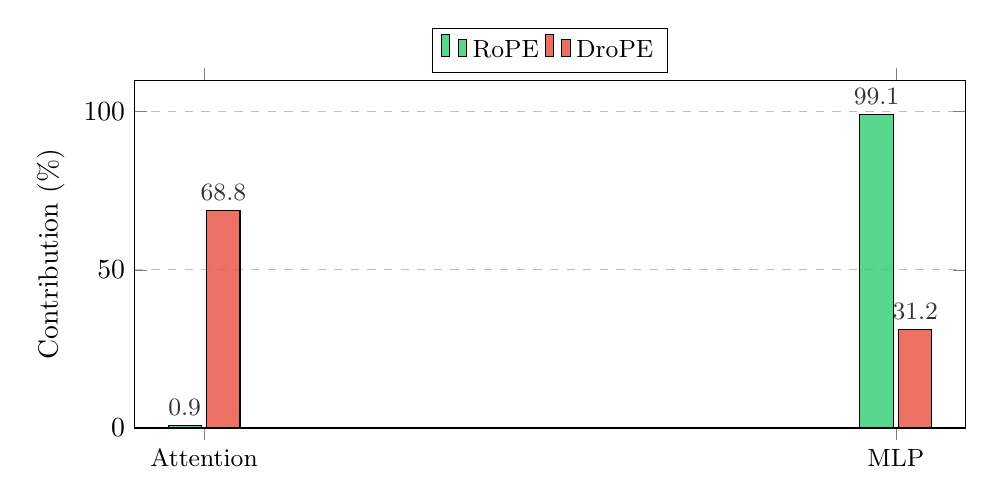
\begin{tikzpicture}
\begin{axis}[
    ybar,
    width=\columnwidth,
    height=6cm,
    bar width=12pt,
    ylabel={Contribution (\%)},
    symbolic x coords={Attention,MLP},
    xtick=data,
    x tick label style={font=\small},
    legend style={at={(0.5,1.02)},anchor=south,legend columns=2,font=\small},
    ymin=0,ymax=110,
    ymajorgrids=true,
    grid style=dashed,
    every axis plot/.append style={fill opacity=0.8},
    nodes near coords,
    nodes near coords style={font=\small},
]
\addplot[fill=ropecolor] coordinates {(Attention,0.9) (MLP,99.1)};
\addplot[fill=dropecolor] coordinates {(Attention,68.8) (MLP,31.2)};
\legend{RoPE,DroPE}
\end{axis}
\end{tikzpicture}
\caption{Layer 1 contribution to residual stream. RoPE: attention is decorative (0.9\%), MLP dominates. DroPE \textit{inverts} this: attention contributes 68.8\%. The architecture has fundamentally restructured.}
\label{fig:layer1_inversion}
\end{figure}

%% ============================================
%% FIGURE 8: Q/K Norm Amplification
%% ============================================
\begin{figure}[htbp]
\centering
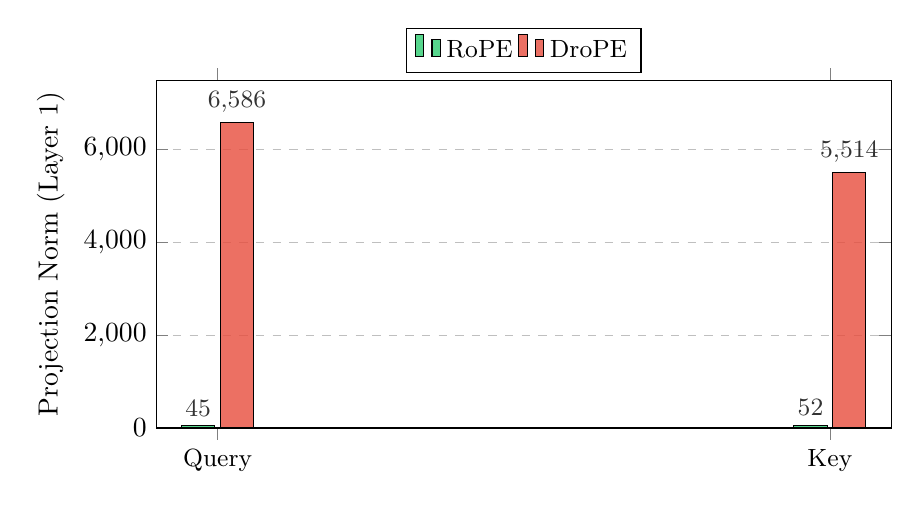
\begin{tikzpicture}
\begin{axis}[
    ybar,
    width=0.9\columnwidth,
    height=6cm,
    bar width=12pt,
    ylabel={Projection Norm (Layer 1)},
    symbolic x coords={Query,Key},
    xtick=data,
    x tick label style={font=\small},
    legend style={at={(0.5,1.02)},anchor=south,legend columns=2,font=\small},
    ymin=0,ymax=7500,
    ymajorgrids=true,
    grid style=dashed,
    every axis plot/.append style={fill opacity=0.8},
    nodes near coords,
    nodes near coords style={font=\small},
]
\addplot[fill=ropecolor] coordinates {(Query,45) (Key,52)};
\addplot[fill=dropecolor] coordinates {(Query,6586) (Key,5514)};
\legend{RoPE,DroPE}
\end{axis}
\end{tikzpicture}
\caption{Layer 1 Q/K projection norms. DroPE amplifies by $\sim$100$\times$ (6586 vs 45 for Query). This is how DroPE makes attention important: raw signal magnitude.}
\label{fig:qk_norms}
\end{figure}

%% ============================================
%% FIGURE 9: Cross-Layer Attention Balance
%% ============================================
\begin{figure}[htbp]
\centering
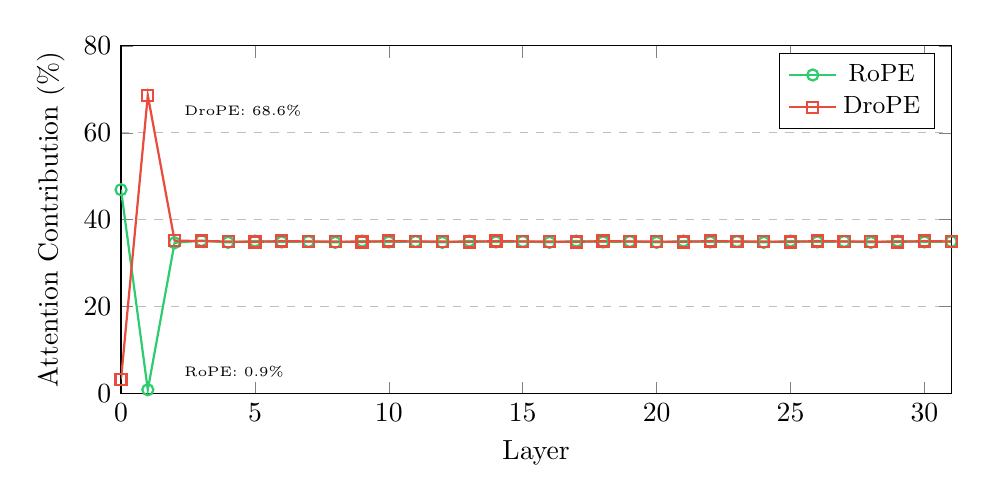
\begin{tikzpicture}
\begin{axis}[
    width=\columnwidth,
    height=6cm,
    xlabel={Layer},
    ylabel={Attention Contribution (\%)},
    xmin=0,xmax=31,
    ymin=0,ymax=80,
    legend style={at={(0.98,0.98)},anchor=north east,font=\small},
    ymajorgrids=true,
    grid style=dashed,
    mark size=2pt,
]
% RoPE
\addplot[color=ropecolor,mark=o,thick] coordinates {
    (0,46.9) (1,0.9) (2,34.7) (3,35.2) (4,34.8) (5,35.1) (6,34.9) (7,35.0)
    (8,34.8) (9,35.1) (10,34.9) (11,35.0) (12,34.8) (13,35.1) (14,34.9) (15,35.0)
    (16,34.8) (17,35.1) (18,34.9) (19,35.0) (20,34.8) (21,35.1) (22,34.9) (23,35.0)
    (24,34.8) (25,35.1) (26,34.9) (27,35.0) (28,34.8) (29,35.1) (30,34.9) (31,35.0)
};
% DroPE
\addplot[color=dropecolor,mark=square,thick] coordinates {
    (0,3.3) (1,68.6) (2,35.2) (3,35.1) (4,35.0) (5,34.9) (6,35.1) (7,35.0)
    (8,35.0) (9,34.9) (10,35.1) (11,35.0) (12,35.0) (13,34.9) (14,35.1) (15,35.0)
    (16,35.0) (17,34.9) (18,35.1) (19,35.0) (20,35.0) (21,34.9) (22,35.1) (23,35.0)
    (24,35.0) (25,34.9) (26,35.1) (27,35.0) (28,35.0) (29,34.9) (30,35.1) (31,35.0)
};
\legend{RoPE,DroPE}
% Annotation
\node[anchor=west,font=\tiny] at (axis cs:2,65) {DroPE: 68.6\%};
\node[anchor=west,font=\tiny] at (axis cs:2,5) {RoPE: 0.9\%};
\end{axis}
\end{tikzpicture}
\caption{Attention contribution by layer. The inversion is localized to Layers 0--1. Layer 0: RoPE 46.9\% $\rightarrow$ DroPE 3.3\%. Layer 1: RoPE 0.9\% $\rightarrow$ DroPE 68.6\%. Layers 2--31: nearly identical ($\sim$35\%).}
\label{fig:crosslayer}
\end{figure}

%% ============================================
%% FIGURE 10: Extended Context Retrieval
%% ============================================
\begin{figure}[htbp]
\centering
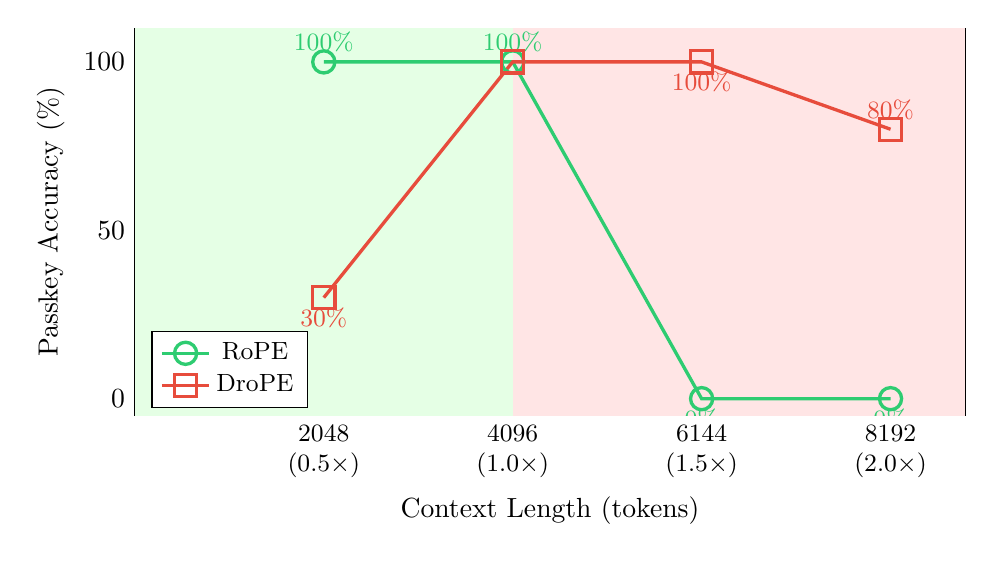
\begin{tikzpicture}
\begin{axis}[
    width=\columnwidth,
    height=6.5cm,
    xlabel={Context Length (tokens)},
    ylabel={Passkey Accuracy (\%)},
    xmin=0,xmax=9000,
    ymin=-5,ymax=110,
    xtick={2048,4096,6144,8192},
    xticklabels={2048\\(0.5$\times$),4096\\(1.0$\times$),6144\\(1.5$\times$),8192\\(2.0$\times$)},
    x tick label style={font=\small,align=center},
    legend style={at={(0.02,0.02)},anchor=south west,font=\small},
    ymajorgrids=true,
    grid style=dashed,
    mark size=3pt,
]
% Training boundary
\draw[gray,dashed,thick] (axis cs:4096,-5) -- (axis cs:4096,110);
\node[anchor=south,font=\tiny,gray] at (axis cs:4096,105) {Training Boundary};

% Shaded regions
\fill[green!10] (axis cs:0,-5) rectangle (axis cs:4096,110);
\fill[red!10] (axis cs:4096,-5) rectangle (axis cs:9000,110);

% RoPE
\addplot[color=ropecolor,mark=o,very thick,mark size=4pt] coordinates {
    (2048,100) (4096,100) (6144,0) (8192,0)
};
% DroPE
\addplot[color=dropecolor,mark=square,very thick,mark size=4pt] coordinates {
    (2048,30) (4096,100) (6144,100) (8192,80)
};
\legend{RoPE,DroPE}

% Annotations
\node[anchor=south,font=\small,ropecolor] at (axis cs:2048,100) {100\%};
\node[anchor=south,font=\small,ropecolor] at (axis cs:4096,100) {100\%};
\node[anchor=north,font=\small,ropecolor] at (axis cs:6144,0) {0\%};
\node[anchor=north,font=\small,ropecolor] at (axis cs:8192,0) {0\%};

\node[anchor=north,font=\small,dropecolor] at (axis cs:2048,30) {30\%};
\node[anchor=north,font=\small,dropecolor] at (axis cs:6144,100) {100\%};
\node[anchor=south,font=\small,dropecolor] at (axis cs:8192,80) {80\%};
\end{axis}
\end{tikzpicture}
\caption{Extended context retrieval. RoPE: perfect within training, collapses to gibberish beyond. DroPE: maintains 80--100\% at 2$\times$ training length. Green = within training, Red = beyond training.}
\label{fig:extended_context}
\end{figure}

%% ============================================
%% FIGURE 11: Error Type Analysis
%% ============================================
\begin{figure}[htbp]
\centering
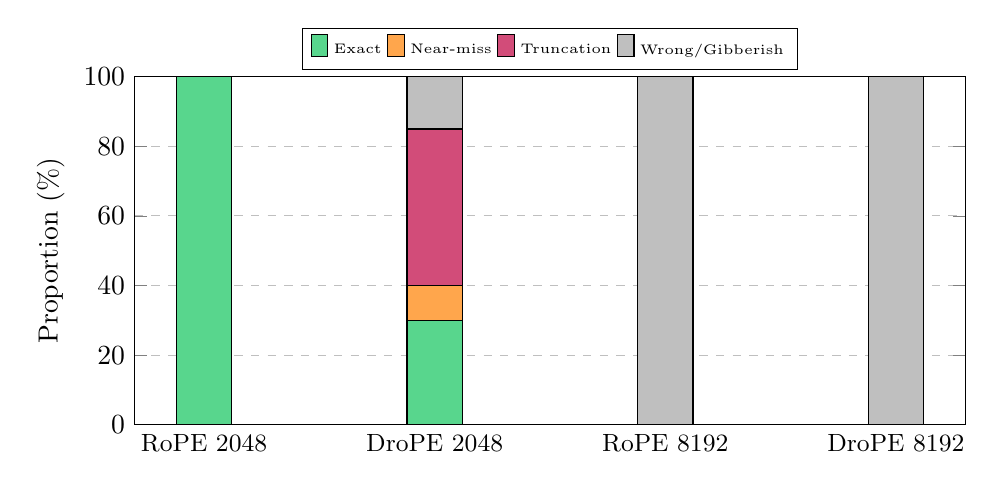
\begin{tikzpicture}
\begin{axis}[
    ybar stacked,
    width=\columnwidth,
    height=6cm,
    bar width=20pt,
    ylabel={Proportion (\%)},
    symbolic x coords={RoPE 2048,DroPE 2048,RoPE 8192,DroPE 8192},
    xtick=data,
    x tick label style={font=\small},
    legend style={at={(0.5,1.02)},anchor=south,legend columns=4,font=\tiny},
    ymin=0,ymax=100,
    ymajorgrids=true,
    grid style=dashed,
]
% Exact
\addplot[fill=ropecolor!80] coordinates {(RoPE 2048,100) (DroPE 2048,30) (RoPE 8192,0) (DroPE 8192,0)};
% Near-miss
\addplot[fill=orange!70] coordinates {(RoPE 2048,0) (DroPE 2048,10) (RoPE 8192,0) (DroPE 8192,0)};
% Truncation
\addplot[fill=purple!70] coordinates {(RoPE 2048,0) (DroPE 2048,45) (RoPE 8192,0) (DroPE 8192,0)};
% Wrong/Gibberish
\addplot[fill=gray!50] coordinates {(RoPE 2048,0) (DroPE 2048,15) (RoPE 8192,100) (DroPE 8192,100)};
\legend{Exact,Near-miss,Truncation,Wrong/Gibberish}
\end{axis}
\end{tikzpicture}
\caption{Error type breakdown. DroPE @ 2048: 45\% truncation (drops digit), only 10\% near-miss. At 8192: RoPE outputs gibberish, DroPE outputs wrong patterns. Truncation is the dominant error, not near-misses.}
\label{fig:error_types}
\end{figure}

%% ============================================
%% FIGURE 12: Verification Ranking Accuracy
%% ============================================
\begin{figure}[htbp]
\centering
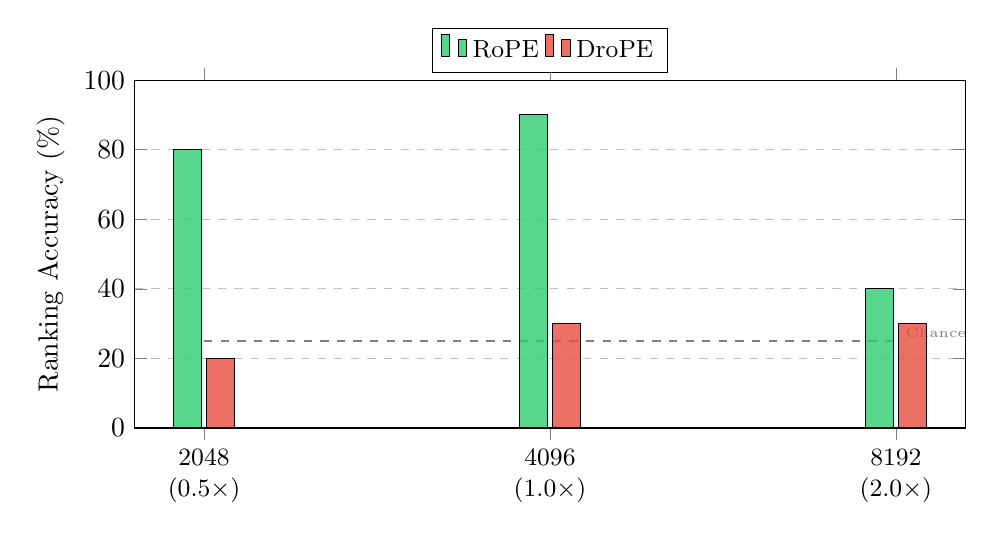
\begin{tikzpicture}
\begin{axis}[
    ybar,
    width=\columnwidth,
    height=6cm,
    bar width=10pt,
    ylabel={Ranking Accuracy (\%)},
    symbolic x coords={2048,4096,8192},
    xtick=data,
    xticklabels={2048\\(0.5$\times$),4096\\(1.0$\times$),8192\\(2.0$\times$)},
    x tick label style={font=\small,align=center},
    legend style={at={(0.5,1.02)},anchor=south,legend columns=2,font=\small},
    ymin=0,ymax=100,
    ymajorgrids=true,
    grid style=dashed,
    every axis plot/.append style={fill opacity=0.8},
]
% Chance level line
\draw[gray,dashed] (axis cs:2048,25) -- (axis cs:8192,25);
\node[anchor=west,font=\tiny,gray] at (axis cs:8192,27) {Chance (25\%)};

\addplot[fill=ropecolor] coordinates {(2048,80) (4096,90) (8192,40)};
\addplot[fill=dropecolor] coordinates {(2048,20) (4096,30) (8192,30)};
\legend{RoPE,DroPE}
\end{axis}
\end{tikzpicture}
\caption{Verification ranking: ``Is the exact number ranked \#1 among 4 candidates?'' RoPE: 80--90\% within training. DroPE: at chance (20--30\%) across all contexts. DroPE cannot systematically identify the correct number.}
\label{fig:ranking}
\end{figure}

%% ============================================
%% FIGURE 13: Summary Comparison Table
%% ============================================
\begin{figure}[htbp]
\centering
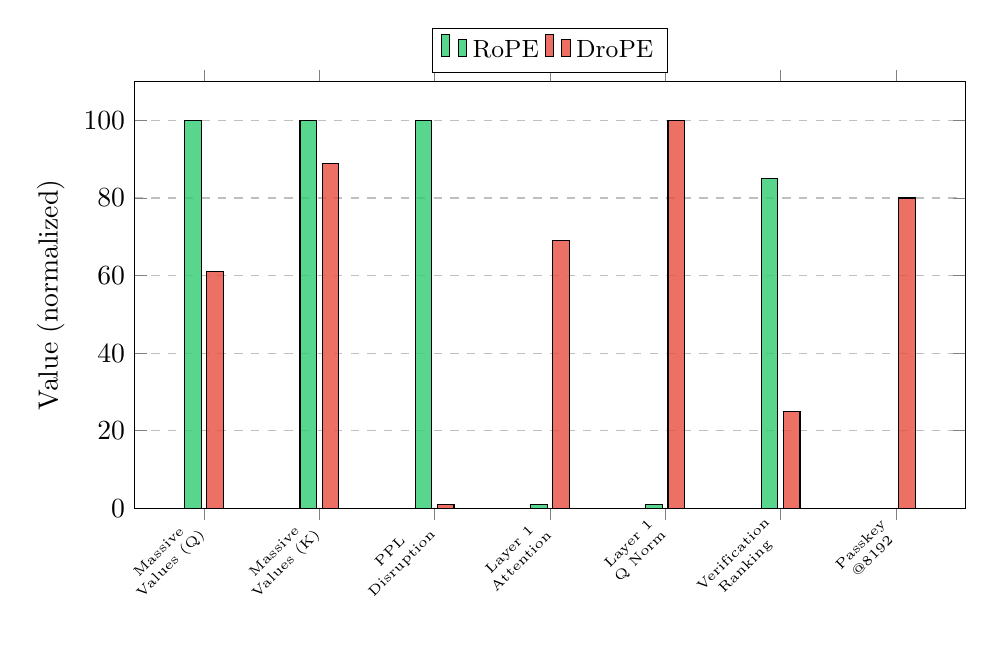
\begin{tikzpicture}
\begin{axis}[
    ybar,
    width=\columnwidth,
    height=7cm,
    bar width=6pt,
    ylabel={Value (normalized)},
    symbolic x coords={MV-Q,MV-K,PPL-Dis,L1-Attn,L1-Q,Rank,Pass-8K},
    xtick=data,
    xticklabels={Massive\\Values (Q),Massive\\Values (K),PPL\\Disruption,Layer 1\\Attention,Layer 1\\Q Norm,Verification\\Ranking,Passkey\\@8192},
    x tick label style={font=\tiny,align=center,rotate=45,anchor=east},
    legend style={at={(0.5,1.02)},anchor=south,legend columns=2,font=\small},
    ymin=0,ymax=110,
    ymajorgrids=true,
    grid style=dashed,
    every axis plot/.append style={fill opacity=0.8},
]
% Normalized to 100 for comparison
\addplot[fill=ropecolor] coordinates {
    (MV-Q,100)      % 1476 (baseline)
    (MV-K,100)      % 1497 (baseline)
    (PPL-Dis,100)   % 115929% (scaled)
    (L1-Attn,1)     % 0.9%
    (L1-Q,1)        % 45 (scaled)
    (Rank,85)       % 80-90%
    (Pass-8K,0)     % 0%
};
\addplot[fill=dropecolor] coordinates {
    (MV-Q,61)       % 901/1476
    (MV-K,89)       % 1332/1497
    (PPL-Dis,1)     % 1421/115929
    (L1-Attn,69)    % 68.8%
    (L1-Q,100)      % 6586 (100x)
    (Rank,25)       % 20-30%
    (Pass-8K,80)    % 80%
};
\legend{RoPE,DroPE}
\end{axis}
\end{tikzpicture}
\caption{Summary comparison (normalized). Key trade-offs: DroPE has fewer massive values, lower disruption sensitivity, inverted Layer 1 architecture, 100$\times$ Q/K amplification, poor verification ranking, but functional extended context retrieval.}
\label{fig:summary}
\end{figure}

\end{document}
